\documentclass[12pt,a4paper,oneside]{article}
\usepackage{amssymb,amsmath,amsthm,amsfonts}
\usepackage[vlined, ruled, linesnumbered]{algorithm2e}
\usepackage{latexsym}
\usepackage{amscd,amsfonts}
\usepackage[OT4]{polski}
\usepackage[utf8]{inputenc}
\usepackage{indentfirst}
\usepackage{graphicx}
\usepackage{float}
\graphicspath{ {images/} }

\begin{document}

\begin{titlepage}
\title{ Kompresja obrazów za pomocą sieci neuronowych typu NEAT - raport}
\maketitle


\begin{flushright}
\author{
\bigskip
Paweł Bielicki
\\Robert Jakubowski}
\end{flushright}

\end{titlepage}

\section{Wstęp}
Dokument przedstawia opis testów przeprowadzonych na programie stworzonym na podstawie dokumentacji wstępnej. W trakcie testów dokonano modyfikacji programu w celu przetestowania możliwości sieci oraz potencjalnemu polepszeniu wyników.

\section{Parametry}
Sieci neuronowe charakteryzują się dużą ilością parametrów. Charakterystyka topologii typu NEAT oraz specyfika problemu kompresji obrazów dodatkowo zwiększają tę ilość. Mnogość parametrów postanowiliśmy ograniczyć do tych, które będą według nas istotne:
\begin{itemize}
	\item inputLayerSize - długość wektora wejściowego,
	\item middleLayerSize - długość wekktora skompresowanego,
	\item numberOfSpecies - liczba osobników w populacji,
	\item maxIteration - maksymalna liczbe iteracji (epok),
	\item maxError - maksymalny dopuszczalny błąd (program zostaje przerwany, gdy błąd sieci jest mniejszy niż maxError),
	\item mutationRatio - współczynnik mutacji,
	\item crossoverRatio - współczynnik krzyżowania.
\end{itemize}

W powyższym zestawieniu istnieje tylko jeden współczynnik do mutacji, który określa z jakim prawdopodobieństwiem mutowany będzie osobnik. Zgodnie z specyfikacją sieć mogła się mutować na kilka sposobów (usuwanie wierzchołka, dodawanie wierzchołka, dodanie połączenia, usunięcie połączenia, zmiana wagi połączenia). Każdy ze sposobów mutacji miał określone własne prawdopodobieństwo ustawione w wyniku przetestowania różnych wariantów. Ostatecznie przyjeliśmy następujące wartości:
\begin{itemize}
\item dodanie połączenia - 0.25,
\item dodanie neuronu - 0.03,
\item usunięcie połączenia - 0.02,
\item zmiana wagi połączenia - 0.67,
\item usunięcie neuronu - 0.03.
\end{itemize}

Do łatwego definiowania nowych testów wykorzystaliśmy narzędzie Gradle.

\section{Wstępne testy i dokonane modyfikacje}
Pierwsza wersja programu dawała wyniki dalekie od oczekiwań. Dla prostych obrazów wyniki były bardzo niedokładne. Nawet dla obrazu, ktory składał się z 2 pasów - czarnego i białego - sieć uczyla się dobrze tylko czarnego koloru, natomiast drugi pasek był jasnoszarym szumem. Dla bardziej skomplikowanych obrazow otrzymywaliśmy obraz, który był szarym szumem. W celu poprawienia wyników zastosowaliśmy nastepujące zmiany w programie:

\begin{enumerate}
\item Usunęliśmy ograniczenie na wagi - mogą przyjmować dowolne wartości, zamiast początkowych wartości z przedziału [0,1]. 
\item Funkcja aktywacji została zamieniona na liniową. 
\item Zmienione zostało parsowanie wyniku sieci na obraz - usunęliśmy dzielenie wartości przez liczbę połączeń neuronu wyjściowego.
\item Powyższe zmiany spowodowały, że wyjście mogło być dowolną liczbą (wcześniej musiała to być liczba z przedziału [0,1]). Zmiana polegała na tym, że wartości spoza przedziału [0,1] są rzutowane na jego ograniczenia.
\\ \\
Zmiany 1-4 spowodowały, że sieć zaczęła wyraźnie zbiegać do oczekiwanych rezultatów. Zauważyliśmy jednak możliwość kolejnych modyfikacji, ponieważ obrazy wyjściowe, w początkowych iteracjach, były białe. Aby temu zaradzić wprowadziliśmy kolejne zmiany:
\\
\item Problem znajdował się w początkowym losowaniu wartości wag. Zmieniliśmy je tak, aby wartością oczekiwaną losowania były wartości, które w efekcie działania sieci dają uśrednianie obrazu. Implementacja polegała na tym, że dla danego połączenia prowadzącego z neuronu A do neuronu B, losowana jest liczba z zakresu [0,2], a następnie dzielona jest przez liczbę połączeń wejściowych neuronu B. Tak otrzymana liczba staje się wagą tego połączenia.

\item Przetestowaliśmy również dobór/zmianę wag z pomocą rozkładu normalnego. Spowodowało, to uśrednienie wartości wyjściowych, przez co dla wejścia/wyjścia o rozmiarze 4 dostajemy dość dobre obrazy wizualne, aczkolwiek po przybliżeniu, widać uśrednienie.

\item Następnie postanowiliśmy poprawić zauważone uśrednianie wyników. Założyliśmy, że to ze względu na sposób liczenia błędu - była to suma kwadratów błędów dla każdego piksela. Ustawiliśmy błąd na prostą sumę błędów, ale to sprawiło, że sieci jeszcze mniej chętniej chciały wychodzić z uśredniania. Spróbowaliśmy więc zastosować liczenie błędu jako sumy czwartych potęg błędów. W ten sposób w początkowych etapach uczenia widać więcej artefaktów, ale sieć szybciej dochodzi do wyszukiwania szczegółów.
\end{enumerate}

\section{Testy}
W tym rozdziale opisane są wykonane testy. W podpisie każdego z obrazów są umieszczone parametry uruchomienia.

W pierwszych testach sprawdziliśmy trywialny przypadek z 4 pikselami:
\begin{figure}[h]
\centering
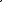
\includegraphics[width=.3\textwidth]{4x4}
\caption{inputLayerSize = 4; middleLayerSize = 1; numberOfSpecies = 50; maxIteration = 1000; maxError = 0.000017; mutationRatio = 0.6; crossoverRatio = 0.1}
\end{figure}
Wynik okazał się identyczny z obrazem wejściowym. Program zakończył swoje dzialania po kilkunastu iteracjach, gdy błąd przekroczył granicę maxError.

Następnie przetestowaliśmy poniższy obraz:

\begin{figure}[h]
\centering

\includegraphics[width=.3\textwidth]{gray2s}
\caption{Obraz wejściowy złożony z dwóch pasków: czarnego i białego o rozmiarze 8x8}
\end{figure}

\begin{figure}[H]
\centering

\includegraphics[width=.3\textwidth]{gray2s-o}
\caption{Obraz wyjściowy. Parametry: inputLayerSize = 64; middleLayerSize = 4; numberOfSpecies = 100; maxIteration = 5000; maxError = 0.00001; mutationRatio = 0.9; crossoverRatio = 0.1}
\end{figure}

Program zakończył się po kilku tysiącach iteracji przekraczając granicę błędu. Mimo małej wartości parametru maxError widać delikatne artefakty. Następne testy przeprowadziliśmy z krótszymi wektorami wejściowymi. Jako obraz testowy wzięliśmy zębatkę:

\begin{figure}[H]
\centering

\includegraphics[width=.4\textwidth]{cog}
\caption{Obraz wejściowy}
\end{figure}

\begin{figure}[H]
\centering

\includegraphics[width=.4\textwidth]{cog4}
\caption{Obraz wyjściowy. Parametry: inputLayerSize = 4; middleLayerSize = 2; numberOfSpecies = 100; maxIteration = 500; maxError = 1; mutationRatio = 0.5; crossoverRatio = 0.1}
\end{figure}

\begin{figure}[H]
\centering

\includegraphics[width=.4\textwidth]{cog16}
\caption{Obraz wyjściowy. Parametry: inputLayerSize = 16; middleLayerSize = 2; numberOfSpecies = 100; maxIteration = 800; maxError = 1; mutationRatio = 0.9; crossoverRatio = 0.1}
\end{figure}

Dla obrazu z inputLayerSize=4 program się skończył, ponieważ granica błędu została przekroczona, natomiast dla drugiego przypadku (z 16 neuronami wejściowymi) po 800 iteracjach błąd wynosił 13.


\section{Podsumowanie}
Wyniki testów pokazują, że założony w dokumentacji wstępnej rozmiar wektora wejściowego (64) jest użyteczny tylko dlla prostych obrazków. Nawet testy z użyciem wektora o długości 16 dały umiarkowane wyniki. Widać z kolei, że testy, w których długość wektora wejściowego jest równa 4 dają dobre rezultaty - nawet dla skomplikowanych obrazów. Warto też zauważyć, że dla tych obrazow w warstwie pośredniej był tylko 1 neuron. Według naszych przewidywań sieć byłaby w stanie się nauczyć trudnych obrazów również dla sieci o większych rozmiarach, ale wymagałoby to dużo dłuższego czasu uczenia.

\end{document}
